\documentclass[tikz, border=6pt]{standalone}
\usepackage{amsmath,amssymb}
\usetikzlibrary{arrows.meta,positioning,calc}
\definecolor{Time}{HTML}{2F80ED}
\definecolor{Space}{HTML}{27AE60}
\definecolor{Union}{HTML}{F2C94C}
\definecolor{Spec}{HTML}{BB6BD9}
\definecolor{Model}{HTML}{EB5757}
\definecolor{Edge}{gray}{0.3}
\begin{document}
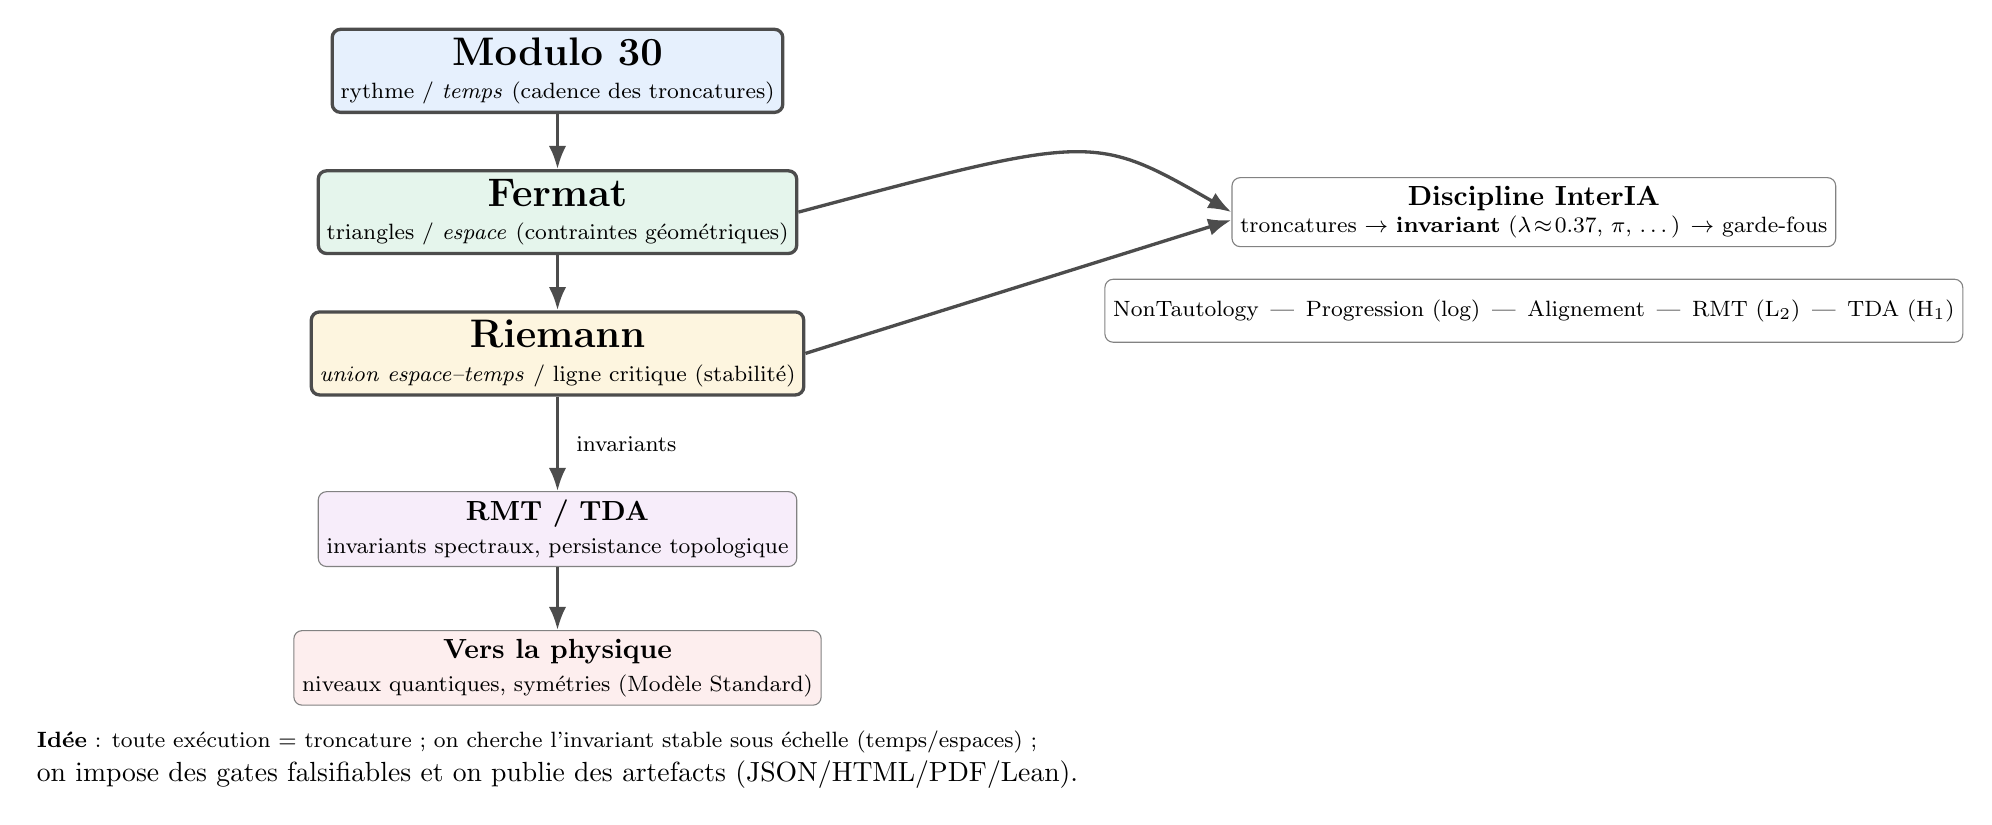
\begin{tikzpicture}[>=Latex, node distance=7mm,
  box/.style={rounded corners=3pt, draw=Edge, very thick, align=center, inner sep=3pt, minimum width=50mm, minimum height=8mm},
  thinbox/.style={rounded corners=3pt, draw=Edge!70, align=center, inner sep=3pt, minimum width=50mm, minimum height=8mm},
  arr/.style={-Latex, very thick, draw=Edge} ]

\node[box, fill=Time!12] (t) {\Large \textbf{Modulo 30}\\ \footnotesize rythme / \emph{temps} (cadence des troncatures)};
\node[box, fill=Space!12, below=of t] (f) {\Large \textbf{Fermat}\\ \footnotesize triangles / \emph{espace} (contraintes g\'eom\'etriques)};
\node[box, fill=Union!18, below=of f] (r) {\Large \textbf{Riemann}\\ \footnotesize \emph{union espace--temps} / ligne critique (stabilit\'e)};

\draw[arr] (t) -- (f);
\draw[arr] (f) -- (r);

\node[thinbox, fill=Spec!12, below=12mm of r] (rmt) {\textbf{RMT / TDA}\\ \footnotesize invariants spectraux, persistance topologique};
\node[thinbox, fill=Model!10, below=8mm of rmt] (ms) {\textbf{Vers la physique}\\ \footnotesize niveaux quantiques, sym\'etries (Mod\`ele Standard)};

\draw[arr] (r) -- node[right, xshift=1mm] {\footnotesize invariants} (rmt);
\draw[arr] (rmt) -- (ms);

\node[thinbox, right=55mm of f, minimum width=62mm] (ia) {\textbf{Discipline InterIA}\\[-2pt] \footnotesize troncatures $\to$ \textbf{invariant} ($\lambda\!\approx\!0.37$, $\pi$, …) $\to$ garde-fous};
\node[thinbox, below=4mm of ia, minimum width=62mm] (guards) {\footnotesize NonTautology \,|\, Progression (log) \,|\, Alignement \,|\, RMT (L$_2$) \,|\, TDA (H$_1$)};

\draw[arr] (f.east) .. controls ($(f.east)!0.5!(ia.west) + (1,1)$) .. (ia.west);
\draw[arr] (r.east) -- ($(ia.west)+(0,-0.1)$);

\node[align=left, below=2mm of ms] (leg) {\footnotesize \textbf{Id\'ee} : toute ex\'ecution = troncature ; on cherche l’invariant stable sous \'echelle (temps/espaces) ;\\ on impose des gates falsifiables et on publie des artefacts (JSON/HTML/PDF/Lean).};

\end{tikzpicture}
\end{document}
